%% 
%% Author:  Olivier Fourmaux (olivier.fourmaux@upmc.fr)
%% 


%%%%%%%%%%%%%%%%%%%%%%%%%%%%%%%%%%%%%%%%%%%%%%%%%%%%%%%%%%%
%% Type et package

\documentclass[a4paper,12pt]{article}

\usepackage[francais,english]{babel}
\usepackage{fancyhdr}
\usepackage[latin1]{inputenc}
\usepackage{epsfig}
\usepackage{calc}
\usepackage{url}
\usepackage{boxedminipage}

%%%%%
%%Rajout
\usepackage{epstopdf}
\usepackage{enumerate}
\usepackage{cite}
\renewcommand{\FrenchLabelItem}{\textbullet}


\newenvironment{changemargin}[2]{%
\begin{list}{}{%
\setlength{\leftmargin}{#1}%
\setlength{\rightmargin}{#2}%
}%
\item[]}
{\end{list}}

%%%%%%%%%%%%%%%%%%%%%%%%%%%%%%%%%%%%%%%%%%%%%%%%%%%%%%%%%%%
%%%%%%%%%%%%%%%%%%%%%%%%%%%%%%%%%%%%%%%%%%%%%%%%%%%%%%%%%%%
%% D�finitions � personnaliser 

%% Pour les noms, utilisez la premi�re lettre du pr�nom suivi du 
%% nom de famille (premi�re lettre majuscule, reste en minuscule).


%%%% Indiquer le nom de l'encadrant ci-dessous:

\def\nomEncad{S.~Secci,\\ Y.~Bencha�b, M.~Coudron}
%%<matthieu.coudron@lip6.fr>,
%%<yacine.benchaib@lip6.fr>
%% Si le projet est co-encadr� indiquer les deux noms � la suite dans 
%% Le m�me champs


%%%% Indiquer les noms des �tudiants participant ci-dessous:

\def\nomEtudC{Q.~Dubois}
\def\nomEtudB{K.~Lam}
\def\nomEtudA{R.~Ly}
\def\nomEtudD{S.~Ravier}

%% Si le projet est encadr� par moins de 4 �tudiants laissez
%% les variables inutiles vides


%%%% Indiquer la r�f�rence (numero) et le nom du sujet ci-dessous:

\def\refProjet{9} \def\titreProjetCourt{perf\,MPTCP\,OpenFlow}
\def\titreProjetLong{MPTCP\\Performances et optimisation de la
  s�curit� avec un ordonnancement r�parti dans les topologies
  virtualis�es OpenFlow}

%% Le titre court ne doit pas faire plus d'une vingtaine de caract�re
%% r�sumez le � quelques mots essenciels


%%%% Indiquer le type de document et sa version ci-dessous:

\def\typeDoc{Cahier Des Charges}
 
%% - Rapport interm�daire
%% - Rapport final



%%%%%%%%%%%%%%%%%%%%%%%%%%%%%%%%%%%%%%%%%%%%%%%%%%%%%%%%%%%
%%%%%%%%%%%%%%%%%%%%%%%%%%%%%%%%%%%%%%%%%%%%%%%%%%%%%%%%%%%
%% D�finitions � ne pas modifier
 
%%%%% ||| Mise en page verticale ||| 
\setlength{\voffset}{-1in} % a4:reste 297mm pour les 5 suivants:
\setlength{\topmargin}{15mm}         % avant l'en-t�te
\setlength{\headheight}{20mm}        % hauteur de l'en-t�te 
\setlength{\headsep}{10mm}            % entre l'en-t�te et le corps
\setlength{\textheight}{220mm}       % hauteur du corps
\setlength{\footskip}{12mm}          % pied de page par rapport au corps 

%%%%% --- Mise en page horizontale ---
\setlength{\hoffset}{-1in} % a4:reste 210mm 
\setlength{\oddsidemargin}{25mm}     % entre hoffset et le corps
\setlength{\evensidemargin}{25mm}    % entre hoffset et le corps
\setlength{\marginparwidth}{0mm}     % largeur de la marge
\setlength{\marginparsep}{0mm}       % s�parateur corps marge
\setlength{\textwidth}{160mm}        % largeur du corps

\def\annee{2013-14}



%%%%%%%%%%%%%%%%%%%%%%%%%%%%%%%%%%%%%%%%%%%%%%%%%%%%%%%%%%%
%% D�but du document

\begin{document}

\selectlanguage{francais}



%%%%%%%%%%%%%%%%%%%%%%%%%%%%%%%%%%%%%%%%%%%%%%%%%%%%%%%%%%%
%% D�finition des en-t�tes et pied de pages
\pagestyle{fancyplain}
\lhead[\fancyplain{}{\texttt{Universit� Pierre et Marie Curie}\\
          Master Informatique\\ UE \textbf{PRes} f�v. \annee \\ \nomEncad}]
      {\fancyplain{}{\textsc{Universit� Pierre et Marie Curie}\\
          Master Informatique\\ UE \textbf{PRes} \annee \\ \nomEncad}}
\chead[\fancyplain{}{\textbf{Projet \refProjet\\\titreProjetCourt}}]
      {\fancyplain{}{\textbf{Projet \refProjet\\\titreProjetCourt}}}
\rhead[\fancyplain{}{\nomEtudA\\\nomEtudB\\\nomEtudC\\\nomEtudD}]
      {\fancyplain{}{\nomEtudA\\\nomEtudB\\\nomEtudC\\\nomEtudD}}
\lfoot[\fancyplain{}{\epsfig{figure=UPMC_sorbonne.eps,width=3cm}}]
      {\fancyplain{}{\epsfig{figure=UPMC_sorbonne.eps,width=3cm}}}
\cfoot[\fancyplain{}{\textbf{\thepage/\pageref{fin}}}]
      {\fancyplain{}{\textbf{\thepage/\pageref{fin}}}}
\rfoot[\fancyplain{}{\typeDoc}]
      {\fancyplain{}{\typeDoc}}

%%%%%%%%%%%%%%%%%%%%%%%%%%%%%%%%%%%%%%%%%%%%%%%%%%%%%%%%%%%

~

      \begin{center}
        \begin{boxedminipage}{12cm}{
            \begin{center}
              ~\\\LARGE\textbf{\titreProjetLong}\\
              ~\\\large Encadrants: \textbf{\nomEncad,}\\
              ~\\\large Etudiants: \textbf{\nomEtudA, \nomEtudB, \nomEtudC, \nomEtudD}\\
              ~
            \end{center}
            }
        \end{boxedminipage}
      \end{center}

~

\tableofcontents
\section{Cahier des charges}

\subsection{Objectifs}
\label{sec:charges:intro}

Les objectifs du projet sont de :
\begin{itemize}
\item mesurer les performances de MPTCP sur diff�rentes topologies de
  r�seaux virtuels.
\item modifier l'ordonnanceur de MPTCP pour privil�gier une
  r�partition �quilibr�e sur les diff�rents sous-flots.
\end{itemize}

\subsection{Contexte}
\label{sec:charges:contexte}

MPTCP est une extension de TCP qui permet pour une connexion TCP
donn�e d'utiliser plusieurs chemins pour l'�change de donn�es. La
multiplicit� des sous-flots a pour but d'am�liorer le d�bit et
d'augmenter la r�silience de la connexion\cite{rfc6182,rfc6824,
  coudroncross2013}.

Les performances de MPTCP ne doivent pas �tre inf�rieures � celles de
TCP et son l'utilisation ne doit pas diminuer le d�bit des autres
utilisateurs s ur le m�me r�seau. Les performances de MPTCP d�pendent
en partie de l'algorithme utilis� pour la r�partition des donn�es
entre les diff�rents sous-flots ouverts \cite{pareto2013}. Pour
caract�riser les performances de l'ordonnanceur de MPTCP, nous allons
le tester dans diff�rents r�seaux virtualis�s en utilisant dans un
premier temps l'algorithme impl�ment� dans le kernel MPTCP de
linux\footnote{\url{mptcp.org}}.

L'emploi de MPTCP am�liorerait la s�curit� si les donn�es transitaient
de mani�re �quilibr�e entre les diff�rents sous-flots, ce qui
complexifient les attaques. Le d�bit global de la connexion serait
affect� car les chemins les plus lents vont ralentir le d�bit des
chemins les plus rapides, ce qui, en contre partie, peut s'av�rer
moins performant qu'une simple connexion TCP.  Nous allons modifier
l'ordonnanceur afin de garantir la r�partition �quitable des charges
puis analyser l'influence de cette modification sur les performances
de MPTCP dans les topologies r�seaux utilis�es pr�c�demment.

\subsection{M�thodes}
\label{sec:charges:methodes}

La r�alisation du projet peut �tre subdivis� en trois parties :
\begin{itemize}
\item la simulation de r�seaux � topologies diff�rentes,
\item l'analyse des performances de MPTCP,
\item l'adaptation de l'ordonnanceur pour l'aspect s�curit�.
\end{itemize}

Nous utiliserons Mininet afin de simuler les topologies r�seaux o�
nous pourrons mesurer les performances de MPTCP � l'aide de l'API
Python fournie par Mininet.  Pour caract�riser l'influence de
l'ordonnanceur sur les performances, nous utiliserons des r�seaux
simples o� les diff�rents sous-flots sont asym�triques et diff�rent
par une propri�t� � la fois : latence, d�bit, pertes... Nous testerons
diff�rents algorithmes de r�partition de charge entre sous-flots :
l'algorithme impl�ment� par d�faut (LIA), celui qui satisfait
l'optimum de pareto par rapport aux objectifs de MPTCP, ou encore un
algorithme de r�partition �quilibr�e de la charge r�seau entre les
diff�rents sous-flots.


\section{Plan de d\'eveloppement}
\label{sec:plan:devt}



La premi�re partie est de consuitre les topologies virtualis�es et de
tester les performances de MTPCP en faisant varier les param�tres des
sous-flots. La seconde partie est de construire un alogrithme
d'ordonnancement r�pondant � des crit�res de s�curit�.
\vspace{0.5cm}

Les �tapes du d�veloppement suivront les points suivants:

\begin{itemize}
\item Pr�paration d'une machine mininet contenant MPTCP pour
  l'ensemble de l'�quipe.
\item Lecture et compr�hension du code de MPTCP et �criture de
  commentaires.
\item Pr�paration de plusieurs topologies : \emph{fat tree} pour
  simuler un \emph{data center} et d'une topologie permettant de
  tester la concurrence entre MPTCP et TCP.
\item Pr�paration d'une biblioth�que de tests et de mesures via l'API python
\item Pr�paration et �criture des algorithmes d'ordonnancement
\item Mesures de performances sur les diff�rents algorithmes
\end{itemize}




\begin{figure}[!htb]
  \begin{changemargin}{-2.0cm}{0.5cm}
    \centering
    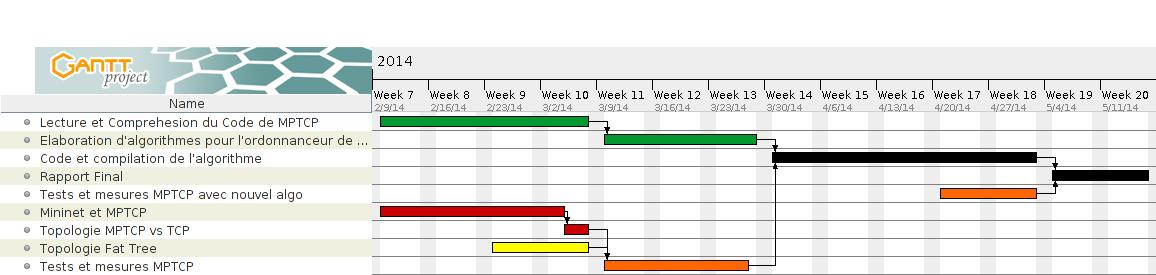
\includegraphics[width=1.2\textwidth]{../gantt/gant.jpg}
  \end{changemargin}
  \centering
  
  \caption{\textbf{Diagramme de Gantt}. Les couleurs correspondent �
    la r�partition grossi�re entre les membres de l'�quipe : en
    \emph{rouge} M. Ly, en \emph{jaune} M. Ravier et en \emph{vert}
    M. Dubois et M. Lam.}
  \label{fig:gantt}
  
\end{figure}



\bibliography{./PRES.bib}
\bibliographystyle{ieeetr}



\label{fin} %% Ne pas supprimer, n�cessaire pour calculer le nombre de pages RL
\end{document}


%%% Local Variables: 
%%% mode: latex
%%% TeX-master: t
%%% End: 
